\documentclass[border=10pt]{article}
%%%<
\usepackage{verbatim}
%%%>
\usepackage{pgfplots}
\pgfplotsset{width=7cm,compat=1.8}
\usepgfplotslibrary{ternary}
\begin{comment}
:Title: A ternary diagram
:Tags: 2D;Ternary diagrams;Manual
:Author: Christian Feuersänger
:Slug: ternary-diagram

The ternary library allows to draw ternary diagrams.
A ternary diagram visualizes three-component systems such that
the sum of them yields 100 percent. Ternary
diagrams are triangular axes.

This example is a (crude) copy of an example of
http://www.sv.vt.edu/classes/MSE2094_NoteBook/96ClassProj/experimental/ternary2.html
and uses area style to change cycle list and the legend appearance.

The code is from the PGFPlots 1.10 manual: "5.12 Ternary Diagrams".
\end{comment}
\begin{document}
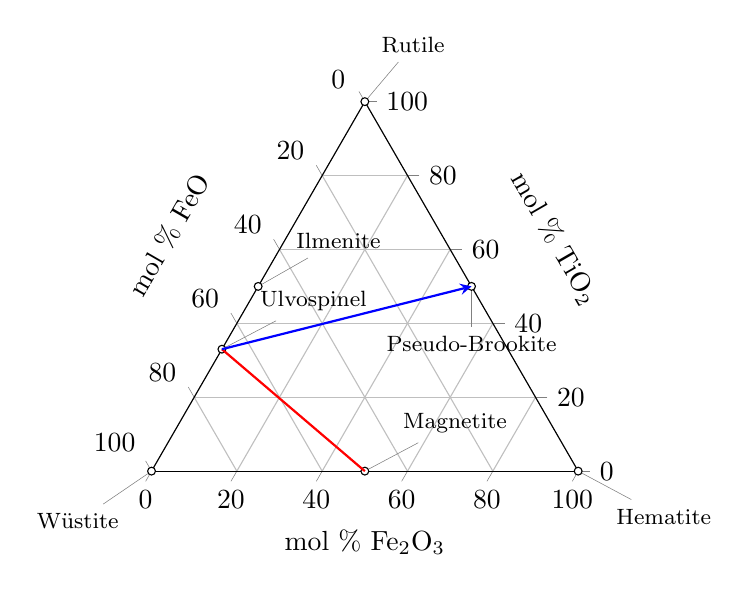
\begin{tikzpicture}
\begin{ternaryaxis}[
	title=,
	xlabel= mol \% TiO$_2$,
	ylabel=mol \% FeO,
	zlabel= mol \% Fe$_2$O$_3$,
	label style=sloped,
	clip=false,
]
node [draw, fill = white] at (0,0,1) {Rutile};	
\node[inner sep=1pt,circle,draw,fill=white,
	  pin=80:\footnotesize Rutile] at (axis cs:1,0,0) {};

\node[inner sep=1pt,circle,draw,fill=white,
	  pin=-125:\footnotesize W\"ustite] at (axis cs:0, 1,0) {};

\node[inner sep=1pt,circle,draw,fill=white,
	  pin=-45:\footnotesize Hematite] at (axis cs:0, 0,1) {};

\node[inner sep=1pt,circle,draw,fill=white,
	  pin=45:\footnotesize Magnetite] at (axis cs:0, 0.5, 0.5) {};
	
\node[inner sep=1pt,circle,draw,fill=white,
	  pin=45:\footnotesize Ilmenite] at (axis cs:0.5, 0.5, 0) {};

\node[inner sep=1pt,circle,draw,fill=white,
	  pin=45:\footnotesize Ulvospinel] at (axis cs:0.33, 0.67, 0) {};

\node[inner sep=1pt,circle,draw,fill=white,
	  pin=-90:\footnotesize Pseudo-Brookite] at (axis cs:0.5, 0, 0.5) {};


\draw[red, thick] (axis cs:0, 0.5, 0.5) -- (axis cs:0.33, 0.67, 0);

\draw[blue, thick, -stealth] (axis cs:0.33, 0.67, 0) -- (axis cs:0.5, 0, 0.5);
\end{ternaryaxis}
\end{tikzpicture}
\end{document}
